\chapter{RISC-V} % Main chapter title
\label{RISC-V} % For referencing the chapter elsewhere, use \ref{Chapter1} 

\section{Einleitung}
\emph{RISC-V} ist eine offene Befehlssatzarchitektur, die 2010 von
Entwicklern an der University of California, Berkeley vorgestellt wurde.
Sie liegt derzeit in Version 2.1 vor (\textit{Stand: März 2017}). RISC-V
basiert auf der RISC (reduced instruction set computing) Designphilosophie.

\paragraph{RISC.} Der Grundgedanke von RISC-Architekturen ist, dass ein Maschinenbefehl möglichst wenige Taktzyklen in der Ausführung benötigt. Damit grenzt sich RISC zu CISC (complex instruction set computing)-Systemen ab, die komplexe Instruktionen beinhalten und zum Teil viele Taktzyklen zur Ausführung benötigen können. RISC-Programme bestehen daher üblicherweise aus mehr Maschinenbefehlen, die aber tendenziell schneller abgearbeitet werden.

Auch wenn der Begriff \textit{reduced instruction} sich
eigentlich nicht auf die Menge der verfügbaren Maschineninstruktionen
bezieht, bestehen RISC-Designs in der Praxis dennoch meist aus weniger
Maschinenbefehlen. Außerdem erfordern RISC-Architekturen in der Regel eine weniger komplizierte Verschaltung. \cite{DBLP:conf/sipew/IsenJJ09} Der Vorteil von RISC-Designs ist somit, insbesondere im Hinblick auf dieses Projekt, dass sie einfacher zu implementieren sind.

%----------------------------------------------------------------------------------------
\section{Architektur}
\label{subsec:Register}

\paragraph{Speicherarchitektur.} RISC-V ist als
\textit{load-store}-Architektur entworfen. Arithmetische und logische
Instruktionen greifen daher nicht auf den Speicher zu, stattdessen
werden alle Operanden und Operationsergebnisse in der Registerbank
abgelegt zwischengespeichert.
Speicherzugriffe werden ausschließlich mit speziellen \textit{Load}- bzw. \textit{Store}-Befehlen realisiert.

\paragraph{Register.} Die RISC-V-Spezifikation definiert $31$
Integer-Register $x1 - x31$. Zusätzlich existiert das
\textit{zero}-Register $x0$, das konstant mit dem Wert $0$ belegt ist. RISC-V-Register sind beliebig verwendbare General-Purpose-Register, die sowohl für Daten als auch Adressen vorgesehen sind. Besondere Verwendungen einzelner Register sind lediglich durch Programmierkonventionen beschrieben. Sonstige Register (v. a. Floating-Point-Register) sind für spezielle Befehlssatzerweiterungen vorgesehen, werden aber an dieser Stelle vernachlässigt.

\paragraph{Instruktionslänge.} RISC-V-Maschinenbefehle sind, wie bei
RISC üblich, in einer fixen Länge kodiert. Sie entspricht der Wortbreite
der Prozessorarchitektur. Für RISC-V-Architekturen sind die Wortbreiten
$32, 64$ oder $128$-Bit vorgesehen.

\paragraph{Byte-Order.} Die RISC-V-Architektur verwendet Little-Endian-Kodierung.
%----------------------------------------------------------------------------------------

%----------------------------------------------------------------------------------------
\section{RISC-V-Varianten}
\label{sec:erweiterung}

\paragraph{Erweiterbarkeit.} Die RISC-V-Architektur ist darauf ausgelegt, flexibel erweiterbar zu sein. Die Spezifikation definiert daher mehrere Teilmengen des Befehlssatzes. \cite[p. 4]{RISC}

\paragraph{Mindeststandard.} Um die RISC-V-Anforderungen zu erfüllen,
muss eine Implementierung zumindest den Basisbefehlssatz umsetzen
(Bezeichnung nach \mbox{RISC-V}-Konvention: \textit{I}). Dieser enthält
neben Befehlen zur Integer-Arithmetik auch Integer Load- und Store-Befehle, sowie die notwendigen Befehle zur Manipulation des Kontrollflusses.

\paragraph{Erweiterungen.} Die allgemeine -- als \textit{General
Purpose} bezeichnete -- Architektur enthält neben diesem Mindeststandard auch Befehle für Gleitkommaarithmetik (F) mit Double (D) oder Quad-Präzision (Q), für die Handhabung verschiedener Privilegierungen (P), für die Verwaltung von Nebenläufigkeit (A) und seit der neusten Version 2.1 auch für Bitmanipulation (B), Vectoroperationen (V) und einigen mehr. \cite[p. 4f.]{RISC}

\paragraph{Umgesetzte Instruktionsmenge.} In diesem Projekt wurde sich
allerdings darauf beschränkt, eine einfache integerverarbeitende
Mikroarchitektur umzusetzen. Als Wortbreite wurde 32-Bit gewählt. Die Bezeichnung des verwendeten Subsets lautet daher nach RISC-V-Konvention \textit{RV32I}. \cite[p. 67ff.]{RISC}
%----------------------------------------------------------------------------------------

%----------------------------------------------------------------------------------------
\section{RV32I}
Das verwendete Subset besteht aus insgesamt $47$ verschiedenen
Maschineninstruktionen. Neben Instruktionen zur Integer-Arithmetik, sind dabei Branch-Instruktionen und Speicherzugriffe enthalten.

\subsection{Instruktionsformate}
RV32I kennt vier verschiedene Typen, in denen Maschineninstruktionen
enkodiert sein können: \textit{R-type}, \textit{I-Type}, \textit{S-type}
und \textit{U-type} - Befehle (siehe Abbildung \ref{fig:instr_types}).
Dabei sind Opcode, sowie Ausgangsregister ($rs1$, $rs2$) und
Zielregister ($rd$) der Operationen immer an der gleichen Stelle des
Maschinenbefehls kodiert. Sofern ein konstanter Wert (\emph{Immediate})
in der Instruktion enthalten ist, ist dieser jeweils in den
höchstwertigst verfügbaren Bits der Instruktion enkodiert. Die Einteilung in 
Instruktionstypen erleichtert die Dekodierung der Instruktionen und führt zu einer simpleren Verschaltung.

\begin{itemize}  
\item Als R-Type sind Register-Instruktionen enkodiert, bei denen beide Operanden in Registern liegen. 
\item Die I-Type-Kodierung ist für Instruktionen vorgesehen, bei denen ein konstanter Wert (\textit{Immediate}) mit einem Wert im Register verrechnet wird.
\item U-Type Befehle umfassen bedingte und unbedingte Sprungbefehle.
\item Der S-Type wird für schreibende Zugriffe auf den Speicher (store) verwendet. 
\end{itemize}

\begin{figure} [h]
  \centering
  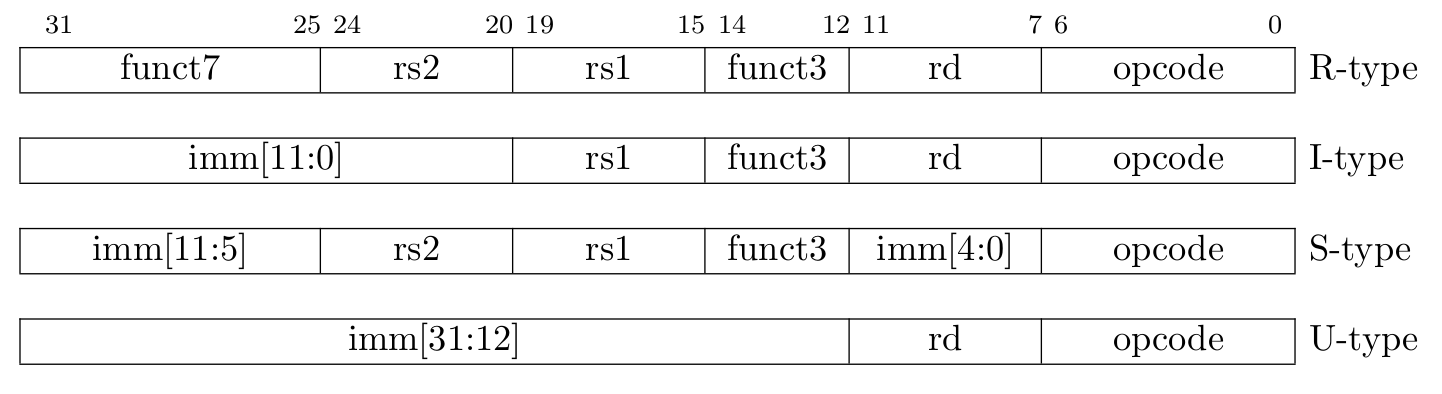
\includegraphics[width=\textwidth]{Figures/instruction_formats}
  \caption{Instruktionsformate. Quelle: \citep[S. 11]{RISC}}
  \label{fig:instr_types}
\end{figure}

\subsection{Immediate-Varianten.} Außerdem existieren mehrere Varianten,
um Immediates aus den Instruktionen zu extrahieren (siehe Abbildung
\ref{fig:immediates}). Diese unterschiedlichen Kodierungen sind ebenfalls so gewählt, um die Überschneidungen der einzelnen Formate zu maximieren und dadurch die Implementierung zu vereinfachen. \cite[S. 11f.]{RISC} 

\begin{figure} [ht]
  \centering
  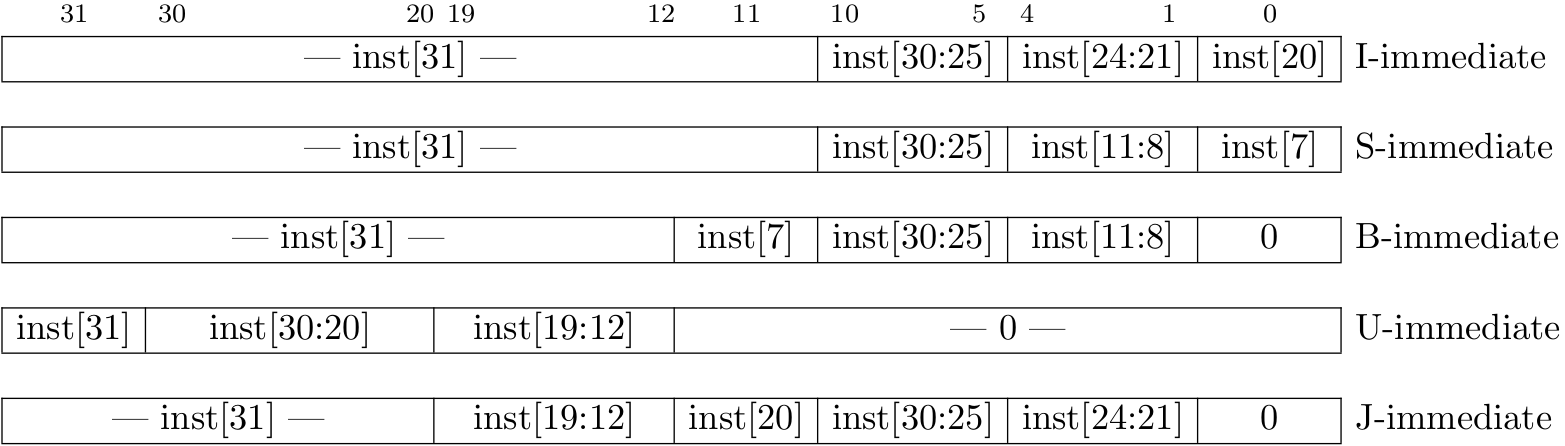
\includegraphics[width=\textwidth]{Figures/immediates}
  \caption{Immediateenkodierungen. Quelle: \citep[S. 12]{RISC}}
  \label{fig:immediates}
\end{figure}

\subsection{Einzelne Instruktionen}
Die in dieser Arbeit umgesetzten Instruktionen des RV32I-Standards können im einzelnen der Tabelle in Anhang \ref{Maschinenbefehle} entnommen werden. Im Folgenden soll lediglich ein Überblick über die Instruktionen dargestellt werden. Ferner wird die Kodierung eines Maschinenbefehls exemplarisch im Detail besprochen.

\paragraph{Integer-Arithmetik.}
Bei integerverarbeitenden Instruktionen kann unterschieden werden zwischen solchen, die eine Operation auf zwei Registerwerten ausführen (als R-Type kodiert) und solchen, die eine Operation auf einem Registerwert und einem Immediate (I-Type) ausführen. Das Operationsergebnis wird jeweils im Zielregister ($rd$) gespeichert.

In den \emph{funct3}- bzw. \emph{funct7}-Bits ist die Operation kodiert,
die auf den Operanden angewendet werden soll. RISC-V definiert
arithmetische Operationen wie die Addition (\emph{ADDI} bzw. \emph{ADD})
und Bitshift-Operationen (\textit{SLL, SRL, SRA}). Außerdem sind
vergleichende Operationen, z. B. Kleiner-Als (\textit{SLT}) vorgesehen,
die eine $1$ im Zielregister ablegt, wenn die Bedingung erfüllt ist,
dass der \emph{rs1}-Registerwert kleiner als der \emph{rs2}-Registerwert
ist. Schließlich sind logische Bitoperationen (\textit{AND, OR, XOR}) definiert.

Es ist außerdem der spezielle \textit{LUI}-Befehl vorgesehen, der
benötigt wird, um 32-Bit-Konstanten in ein Register zu laden. Aufgrund
der festen Instruktionslänge von 32-Bit kann keine ganze
32-Bit-Immediate in einer Instruktion kodiert werden. \textit{LUI} füllt 
deshalb nur die höchstwertigsten 20 Bit eines Wertes und belegt den Rest mit $0$. In einem 
zweiten Schritt kann dann durch eine Veroderung mit dem \textit{ORI}-Befehl der restliche Teil nachgeladen werden.

\paragraph{Beispiel.} In Abbildung \ref{fig:addi} ist exemplarisch der \textit{ADDI}-Befehl zu sehen. Dieser soll einen im Maschinenbefehl kodierten Immediate-Wert mit einem Wert in einem bestimmten Register addieren und das Ergebnis anschließend in einem Zielregister speichern.
 
Dafür ist in der Maschineninstruktion der Opcode $0010011$ (Bit $6 -
0$) kodiert, der die Information enthält, dass eine Immediate-Operation durchgeführt werden soll. Die Bits 14-12 kodieren, die die auszuführende Rechenoperation beschreibt (hier: $000$ für die Addition). Ferner ist das Zielregister $rd$, das Ausgangsregister $rs1$ und der Immediate-Wert (Bit $31 - 20$) im Maschinenbefehl selbst kodiert.

\begin{figure} [ht]
  \centering
  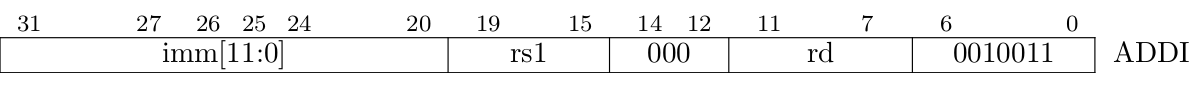
\includegraphics[width=\textwidth]{Figures/ADDI}
  \caption{ADDI-Instruktion.}
  \label{fig:addi}
\end{figure}

\paragraph{Kontrollfluss.}
Um die Reihenfolge, mit der die Maschinenbefehle ausgeführt werden zu
manipulieren, existieren bedingte Sprungbefehle (\textit{BEQ, BNE, BLT,
BGE}). Diese führen einen relativen Sprung an einen Offset von der aktuellen
Adresse des Programmzählers aus, wenn eine bestimmte Bedingung
erfüllt ist, z. B. wenn die Registerinhalte \emph{rs1} und \emph{rs2} gleich sind.

Außerdem existieren unbedingte Sprungbefehle (\textit{JAL, JALR}), die
vor allem zum Aufruf von Subroutinen erforderlich sind. \emph{JAL}
springt ebenfalls den in der Immediate kodierten Offset der aktuellen
Adresse an und speichert
die folgende Maschinenbefehladresse im Zielregister \emph{rd}, um später
wieder zurückkehren zu können. \emph{JALR} springt dagegen eine absolute
Adresse an, die aus dem Immediate-Wert und dem Register \emph{rs1} errechnet wird.

\paragraph{Speicherzugriffe.}
Da RISC-V als Load-Store-Architektur entworfen ist, sind Zugriffe auf den Speicher nur in speziellen Load-/Store-Befehlen vorgesehen. Die \textit{load}-Instruktion lädt einen Wert aus dem Speicher in ein Register, die \textit{store}-Instruktion schreibt einen Registerinhalt an eine bestimmte Speicheradresse. RISC-V erlaubt dabei Zugriffe auf einzelne Byte, Halfwords (2 Byte) und Words (4 Byte).
%----------------------------------------------------------------------------------------

